\documentclass[11pt]{article}
\usepackage[textwidth=18.0cm, textheight=23.0cm, top=2.0cm]{geometry}
\usepackage{pst-all}
\usepackage{amssymb}
\usepackage{tikz}
\usepackage{underscore}\begin{document}
\pagestyle{empty}


ClassName: \underline{\textbf{Class_08.2bp-26}}
\par
BinSize: \underline{\textbf{100 × 100}}
\par
ReduceSize: \underline{\textbf{100 × 100}}
\par
TypeNum: \underline{\textbf{59}}
\par
Num: \underline{\textbf{60}}
\par
OutS: \underline{\textbf{140000}}
\par
InS: \underline{\textbf{121459}}
\par
Rate: \underline{\textbf{0.868}}
\par
UB: \underline{\textbf{14}}
\par
LB0: \underline{\textbf{14}}
\par
LB: \underline{\textbf{14}}
\par
LBWithCut: \underline{\textbf{14}}
\par
NodeCut: \underline{\textbf{0}}
\par
ExtendedNodeCnt: \underline{\textbf{1}}
\par
GenNodeCnt: \underline{\textbf{1}}
\par
PrimalNode: \underline{\textbf{0}}
\par
ColumnCount: \underline{\textbf{14}}
\par
TotalCutCount: \underline{\textbf{0}}
\par
RootCutCount: \underline{\textbf{0}}
\par
LPSolverCnt: \underline{\textbf{1}}
\par
PricingSolverCnt: \underline{\textbf{0}}
\par
BranchAndBoundNum: \underline{\textbf{1}}
\par
isOpt: \underline{\textbf{true}}
\par
TimeOnPrimal: \underline{\textbf{0.000 s}}
\par
TimeOnPricing: \underline{\textbf{0.000 s}}
\par
TimeOnRmp: \underline{\textbf{0.063 s}}
\par
TotalTime: \underline{\textbf{0.140 s}}
\par
\newpage


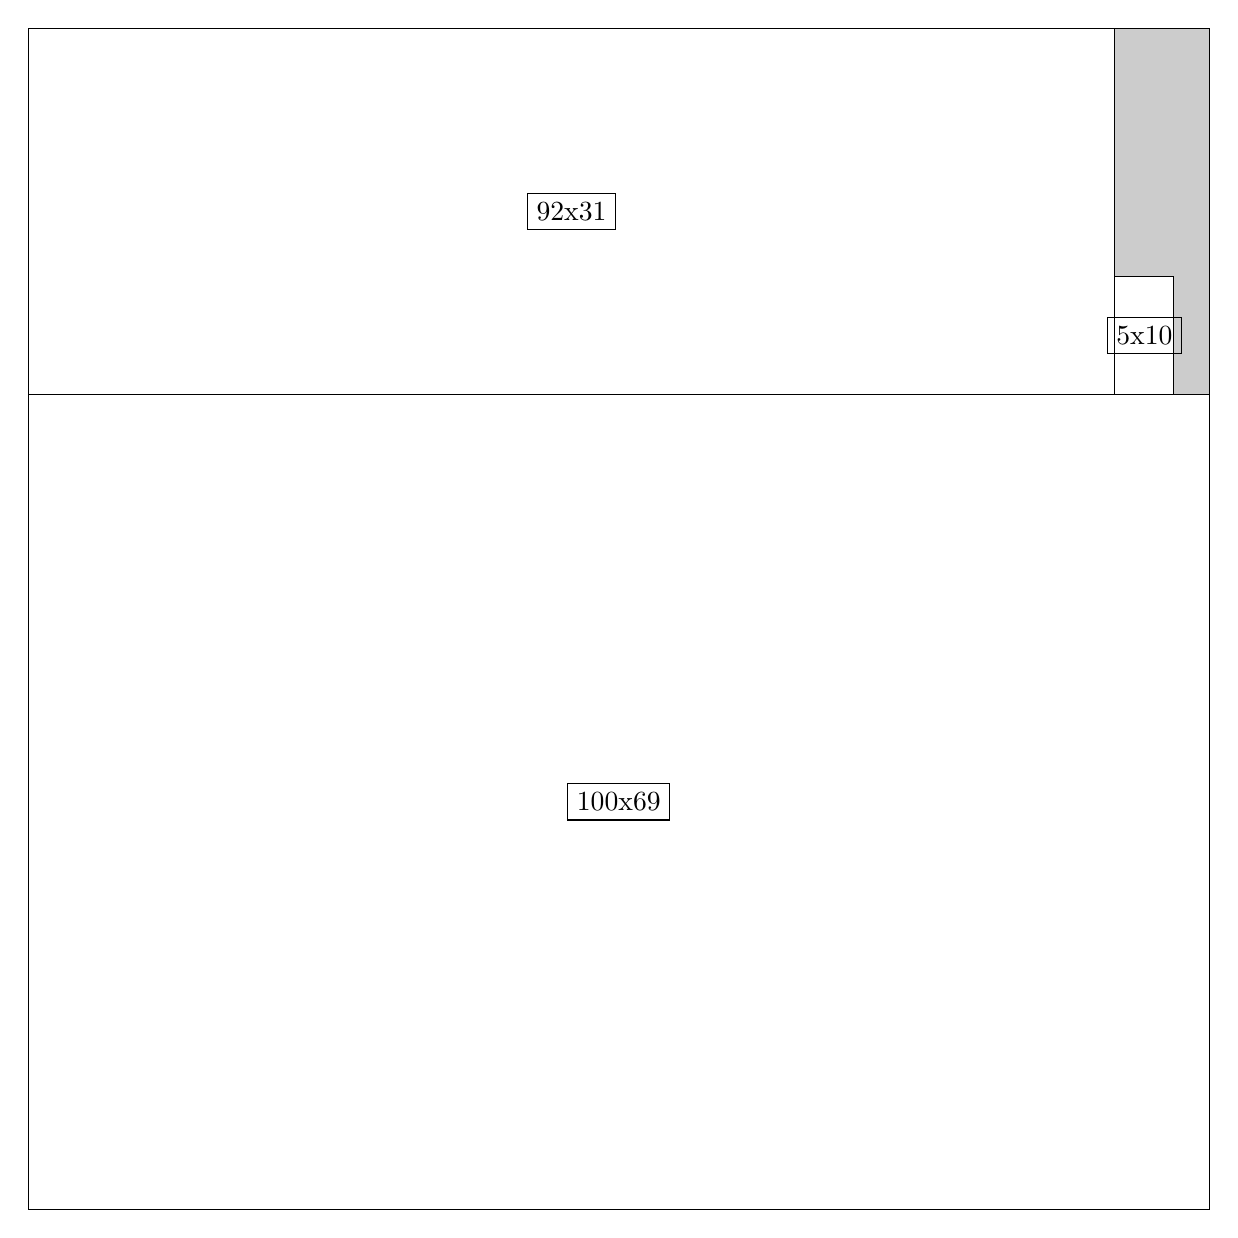
\begin{tikzpicture}[shorten >=1pt,scale=1.0,every node/.style={scale=1.0},->]
\tikzstyle{vertex}=[circle,fill=black!25,minimum size=14pt,inner sep=0pt]
\filldraw[fill=gray!40!white, draw=black] (0,0) rectangle (15.0,15.0);
\foreach \name/\x/\y/\w/\h in {100x69/0.0/0.0/15.0/10.35,92x31/0.0/10.35/13.799999999999999/4.6499999999999995,5x10/13.799999999999999/10.35/0.75/1.5}
\filldraw[fill=white!40!white, draw=black] (\x,\y) rectangle node[draw] (\name) {\name} ++(\w,\h);
\end{tikzpicture}


w =100 , h =69 , x =0 , y =0 , v =6900
\par
w =92 , h =31 , x =0 , y =69 , v =2852
\par
w =5 , h =10 , x =92 , y =69 , v =50
\par
\newpage


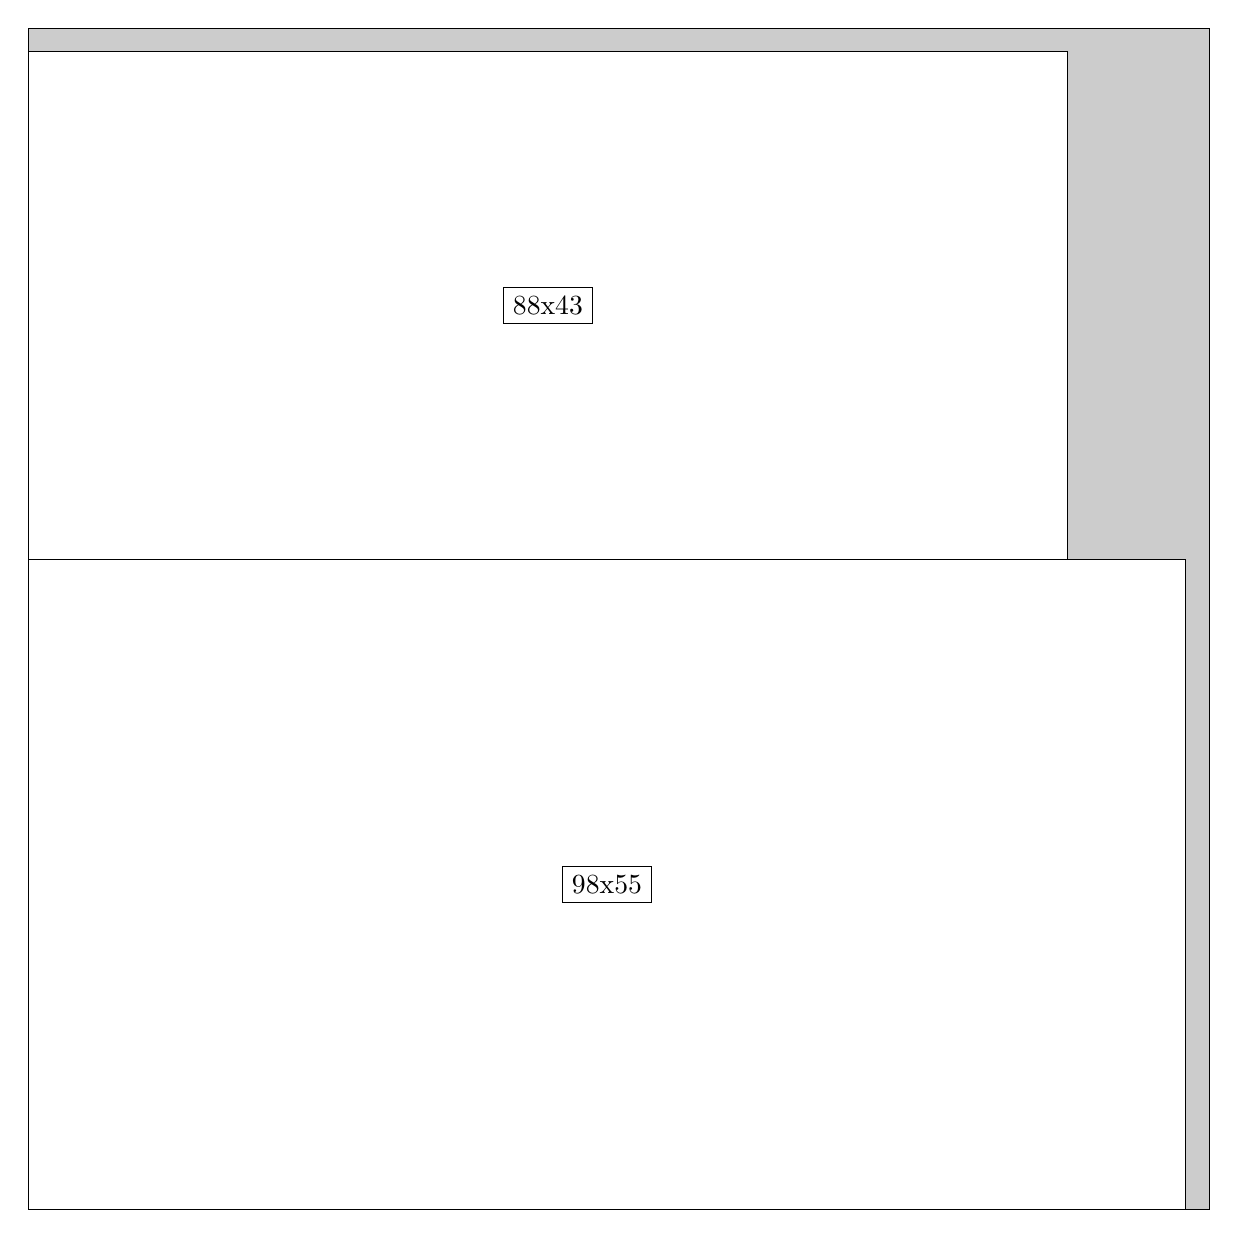
\begin{tikzpicture}[shorten >=1pt,scale=1.0,every node/.style={scale=1.0},->]
\tikzstyle{vertex}=[circle,fill=black!25,minimum size=14pt,inner sep=0pt]
\filldraw[fill=gray!40!white, draw=black] (0,0) rectangle (15.0,15.0);
\foreach \name/\x/\y/\w/\h in {98x55/0.0/0.0/14.7/8.25,88x43/0.0/8.25/13.2/6.45}
\filldraw[fill=white!40!white, draw=black] (\x,\y) rectangle node[draw] (\name) {\name} ++(\w,\h);
\end{tikzpicture}


w =98 , h =55 , x =0 , y =0 , v =5390
\par
w =88 , h =43 , x =0 , y =55 , v =3784
\par
\newpage


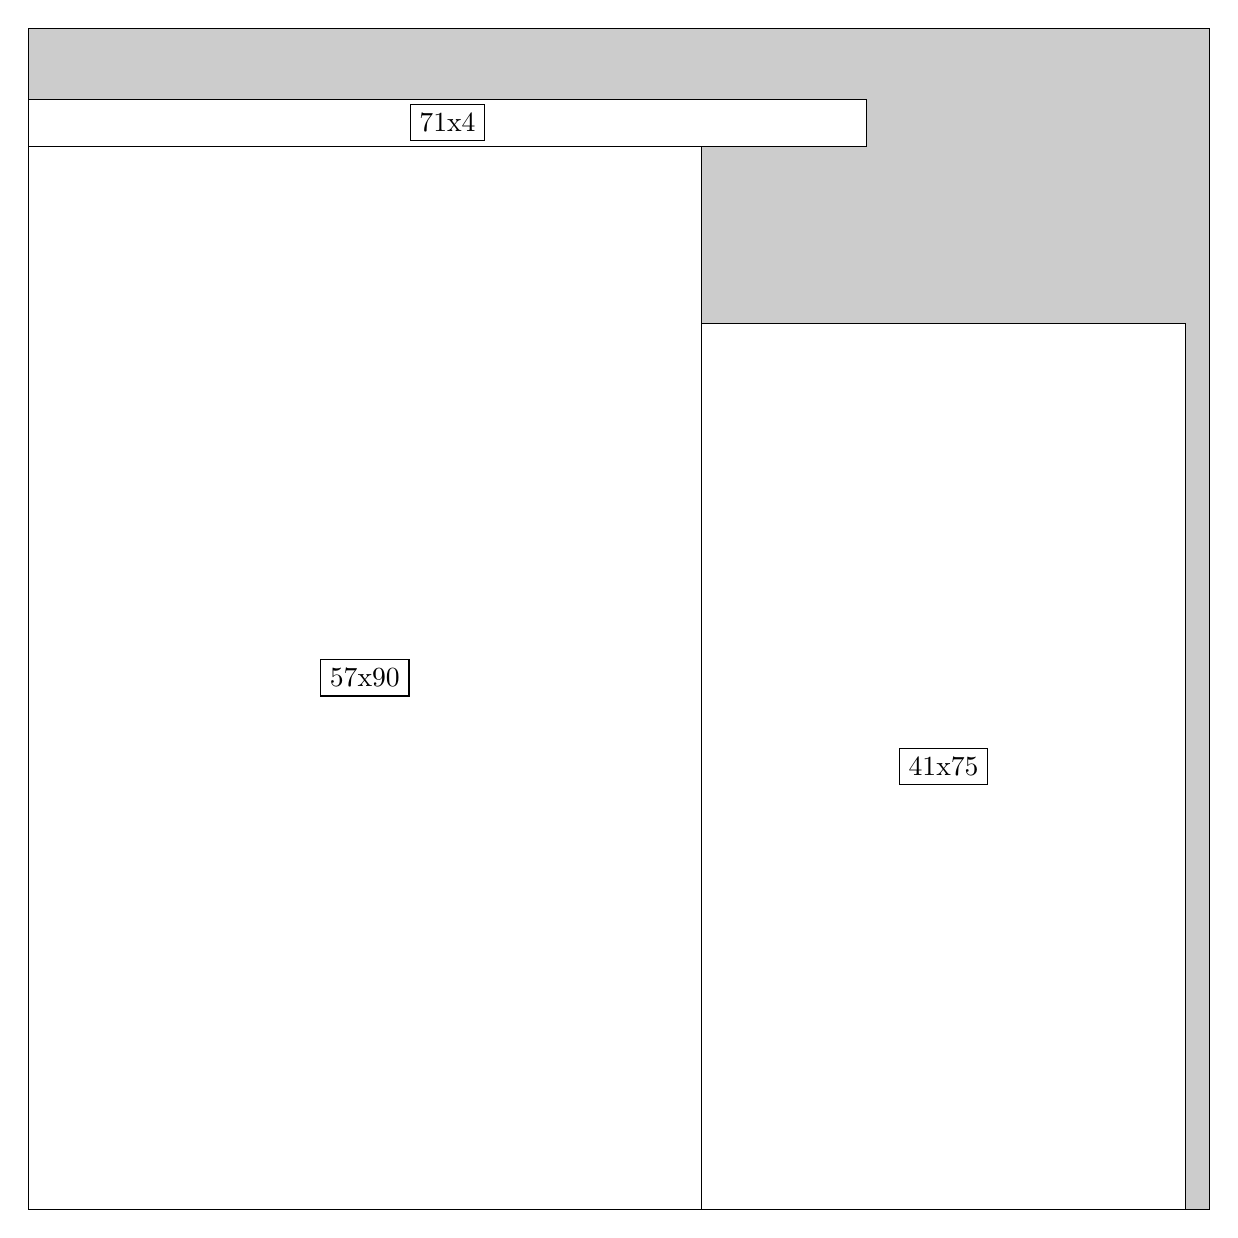
\begin{tikzpicture}[shorten >=1pt,scale=1.0,every node/.style={scale=1.0},->]
\tikzstyle{vertex}=[circle,fill=black!25,minimum size=14pt,inner sep=0pt]
\filldraw[fill=gray!40!white, draw=black] (0,0) rectangle (15.0,15.0);
\foreach \name/\x/\y/\w/\h in {57x90/0.0/0.0/8.549999999999999/13.5,41x75/8.549999999999999/0.0/6.1499999999999995/11.25,71x4/0.0/13.5/10.65/0.6}
\filldraw[fill=white!40!white, draw=black] (\x,\y) rectangle node[draw] (\name) {\name} ++(\w,\h);
\end{tikzpicture}


w =57 , h =90 , x =0 , y =0 , v =5130
\par
w =41 , h =75 , x =57 , y =0 , v =3075
\par
w =71 , h =4 , x =0 , y =90 , v =284
\par
\newpage


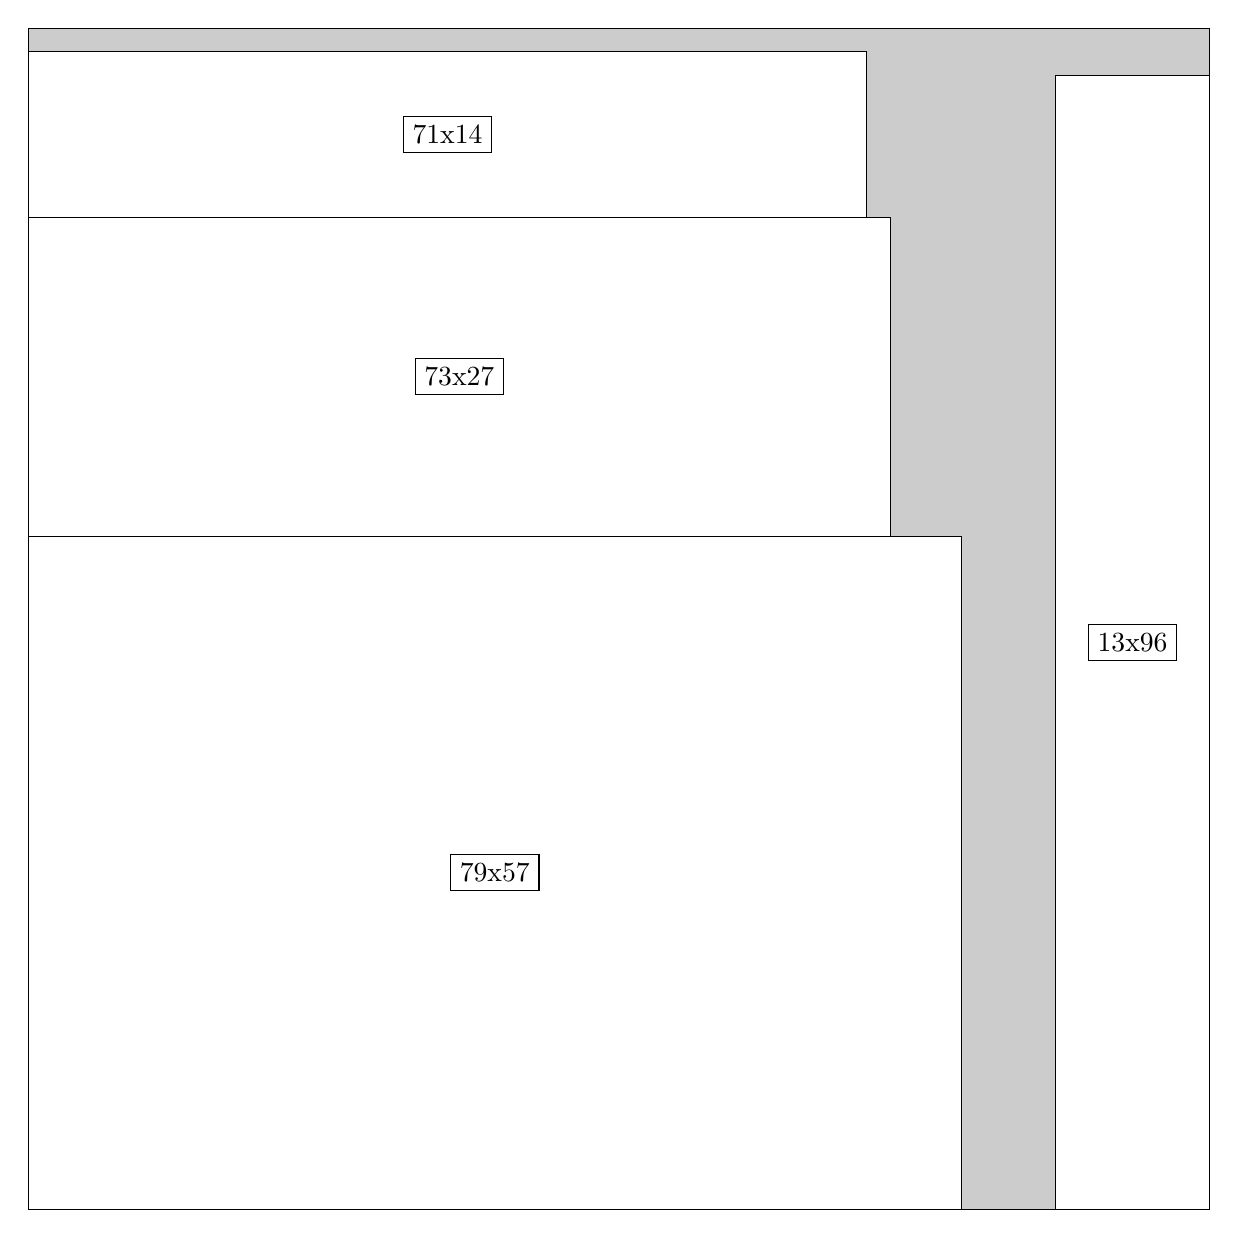
\begin{tikzpicture}[shorten >=1pt,scale=1.0,every node/.style={scale=1.0},->]
\tikzstyle{vertex}=[circle,fill=black!25,minimum size=14pt,inner sep=0pt]
\filldraw[fill=gray!40!white, draw=black] (0,0) rectangle (15.0,15.0);
\foreach \name/\x/\y/\w/\h in {79x57/0.0/0.0/11.85/8.549999999999999,73x27/0.0/8.549999999999999/10.95/4.05,13x96/13.049999999999999/0.0/1.95/14.399999999999999,71x14/0.0/12.6/10.65/2.1}
\filldraw[fill=white!40!white, draw=black] (\x,\y) rectangle node[draw] (\name) {\name} ++(\w,\h);
\end{tikzpicture}


w =79 , h =57 , x =0 , y =0 , v =4503
\par
w =73 , h =27 , x =0 , y =57 , v =1971
\par
w =13 , h =96 , x =87 , y =0 , v =1248
\par
w =71 , h =14 , x =0 , y =84 , v =994
\par
\newpage


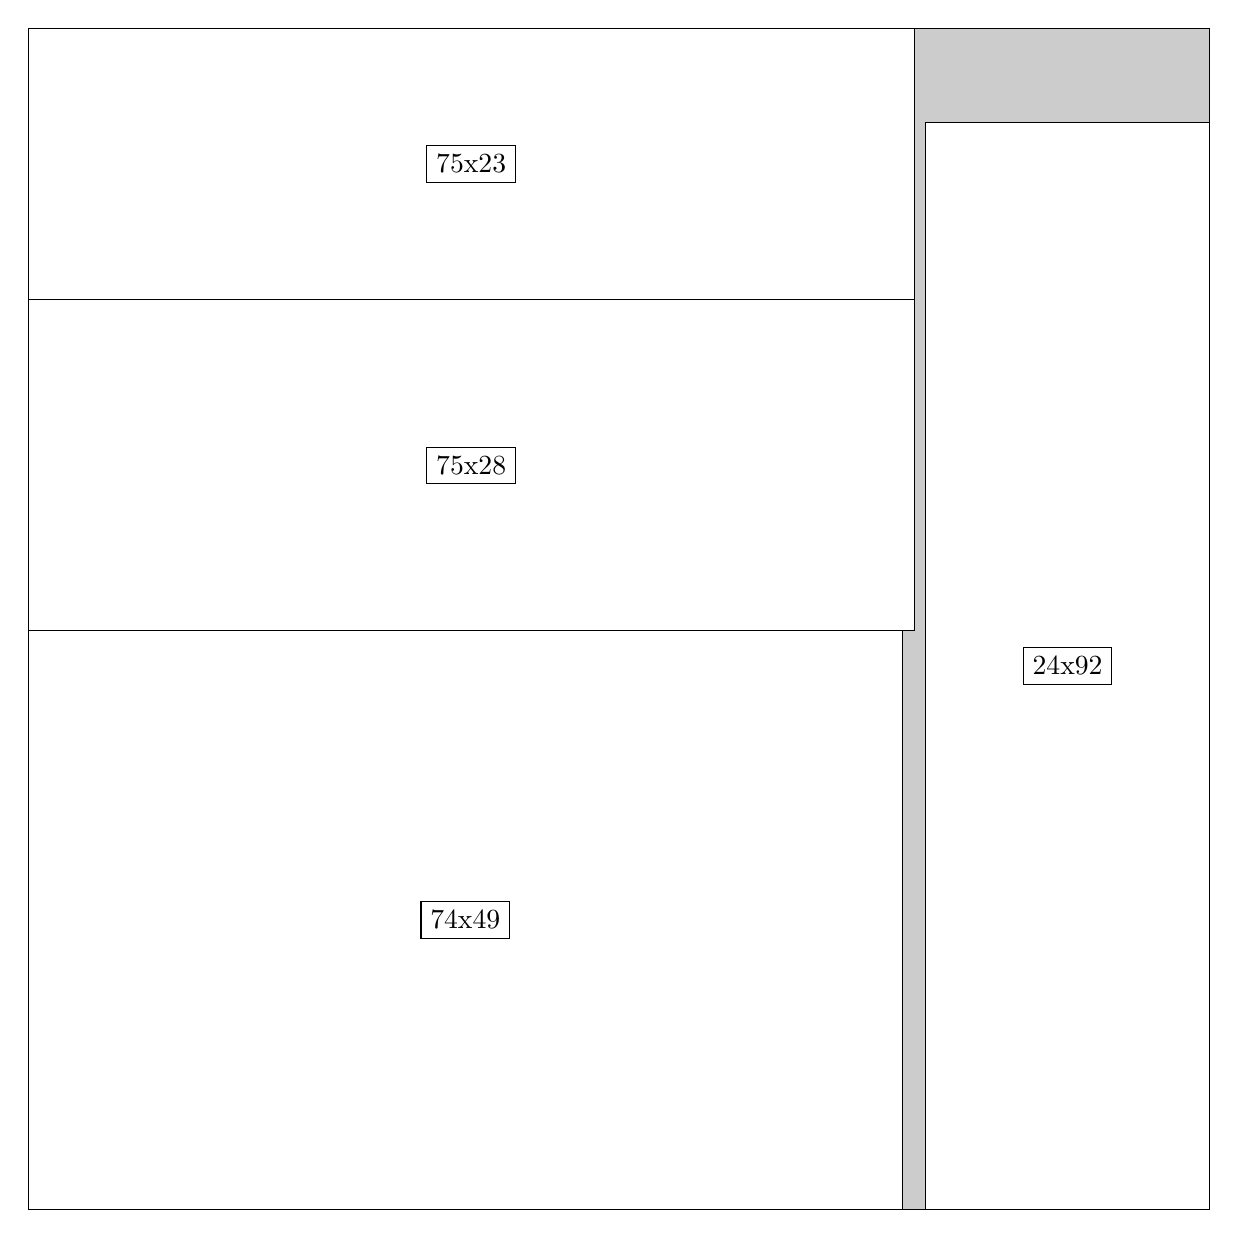
\begin{tikzpicture}[shorten >=1pt,scale=1.0,every node/.style={scale=1.0},->]
\tikzstyle{vertex}=[circle,fill=black!25,minimum size=14pt,inner sep=0pt]
\filldraw[fill=gray!40!white, draw=black] (0,0) rectangle (15.0,15.0);
\foreach \name/\x/\y/\w/\h in {74x49/0.0/0.0/11.1/7.35,24x92/11.4/0.0/3.5999999999999996/13.799999999999999,75x28/0.0/7.35/11.25/4.2,75x23/0.0/11.549999999999999/11.25/3.4499999999999997}
\filldraw[fill=white!40!white, draw=black] (\x,\y) rectangle node[draw] (\name) {\name} ++(\w,\h);
\end{tikzpicture}


w =74 , h =49 , x =0 , y =0 , v =3626
\par
w =24 , h =92 , x =76 , y =0 , v =2208
\par
w =75 , h =28 , x =0 , y =49 , v =2100
\par
w =75 , h =23 , x =0 , y =77 , v =1725
\par
\newpage


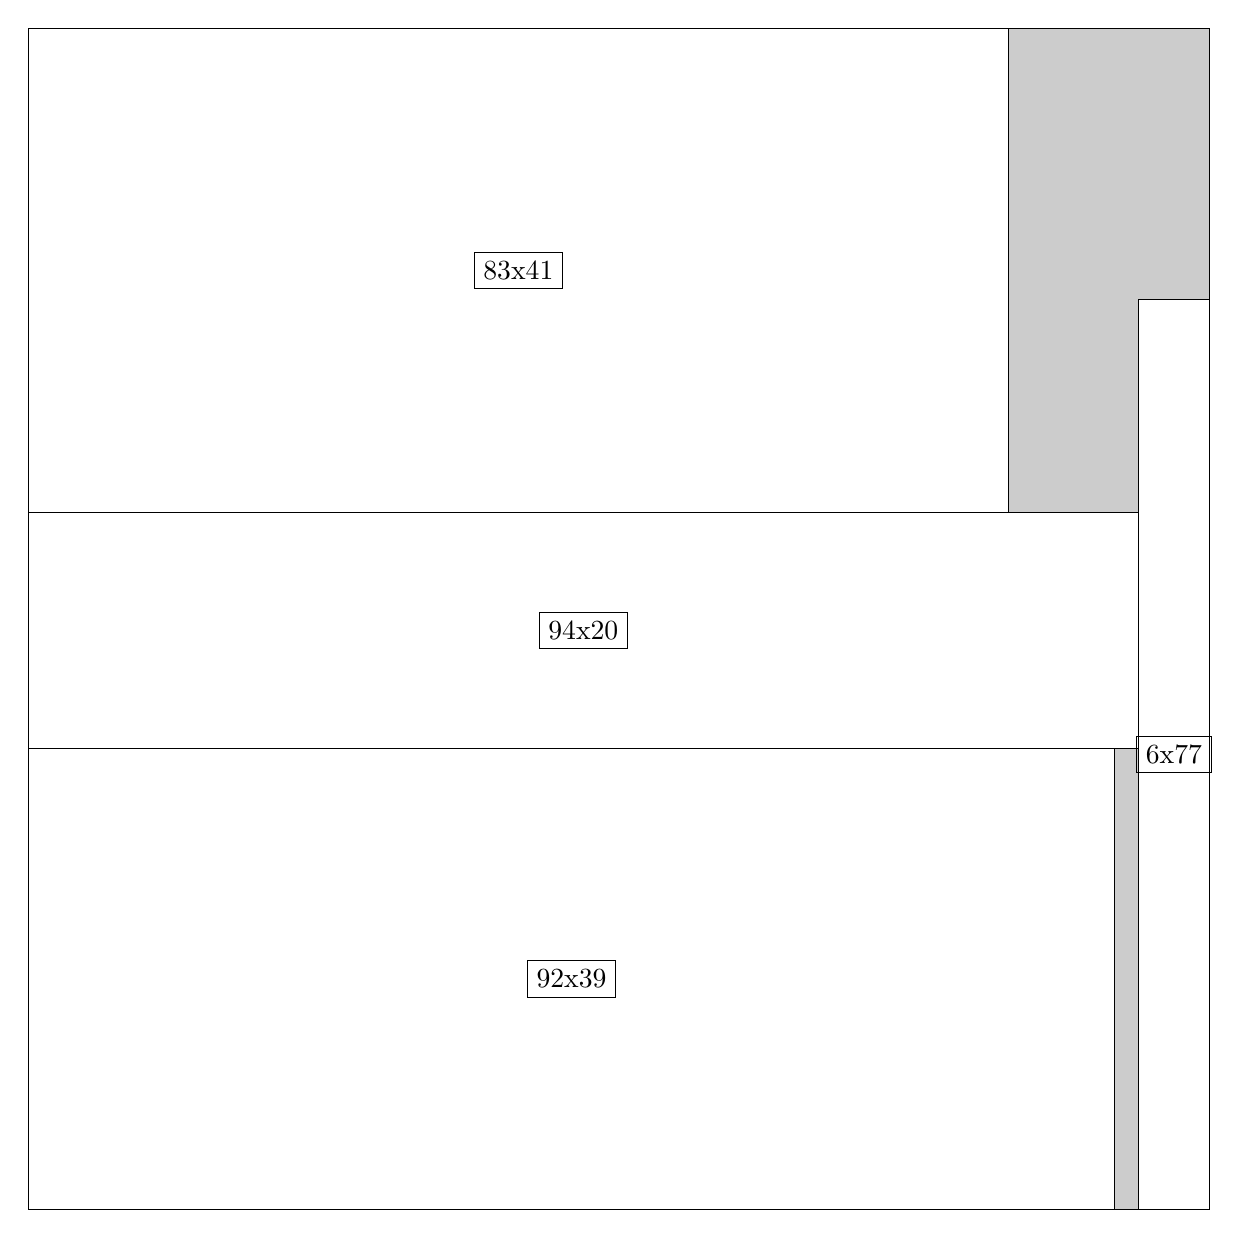
\begin{tikzpicture}[shorten >=1pt,scale=1.0,every node/.style={scale=1.0},->]
\tikzstyle{vertex}=[circle,fill=black!25,minimum size=14pt,inner sep=0pt]
\filldraw[fill=gray!40!white, draw=black] (0,0) rectangle (15.0,15.0);
\foreach \name/\x/\y/\w/\h in {92x39/0.0/0.0/13.799999999999999/5.85,83x41/0.0/8.85/12.45/6.1499999999999995,94x20/0.0/5.85/14.1/3.0,6x77/14.1/0.0/0.8999999999999999/11.549999999999999}
\filldraw[fill=white!40!white, draw=black] (\x,\y) rectangle node[draw] (\name) {\name} ++(\w,\h);
\end{tikzpicture}


w =92 , h =39 , x =0 , y =0 , v =3588
\par
w =83 , h =41 , x =0 , y =59 , v =3403
\par
w =94 , h =20 , x =0 , y =39 , v =1880
\par
w =6 , h =77 , x =94 , y =0 , v =462
\par
\newpage


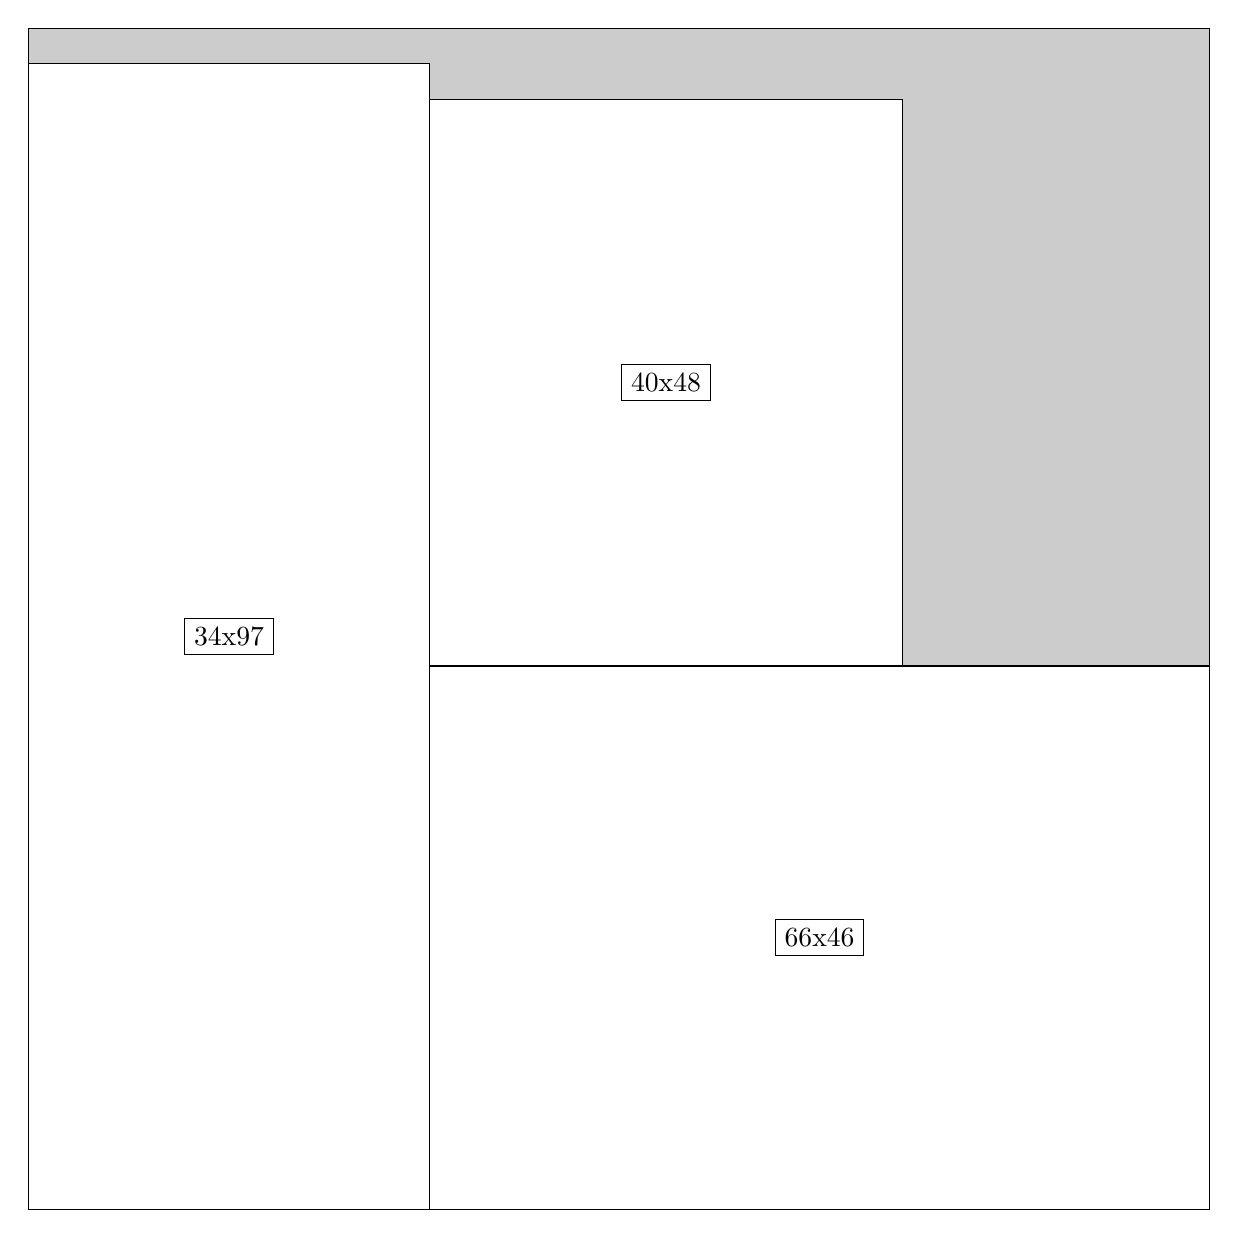
\begin{tikzpicture}[shorten >=1pt,scale=1.0,every node/.style={scale=1.0},->]
\tikzstyle{vertex}=[circle,fill=black!25,minimum size=14pt,inner sep=0pt]
\filldraw[fill=gray!40!white, draw=black] (0,0) rectangle (15.0,15.0);
\foreach \name/\x/\y/\w/\h in {34x97/0.0/0.0/5.1/14.549999999999999,66x46/5.1/0.0/9.9/6.8999999999999995,40x48/5.1/6.8999999999999995/6.0/7.199999999999999}
\filldraw[fill=white!40!white, draw=black] (\x,\y) rectangle node[draw] (\name) {\name} ++(\w,\h);
\end{tikzpicture}


w =34 , h =97 , x =0 , y =0 , v =3298
\par
w =66 , h =46 , x =34 , y =0 , v =3036
\par
w =40 , h =48 , x =34 , y =46 , v =1920
\par
\newpage


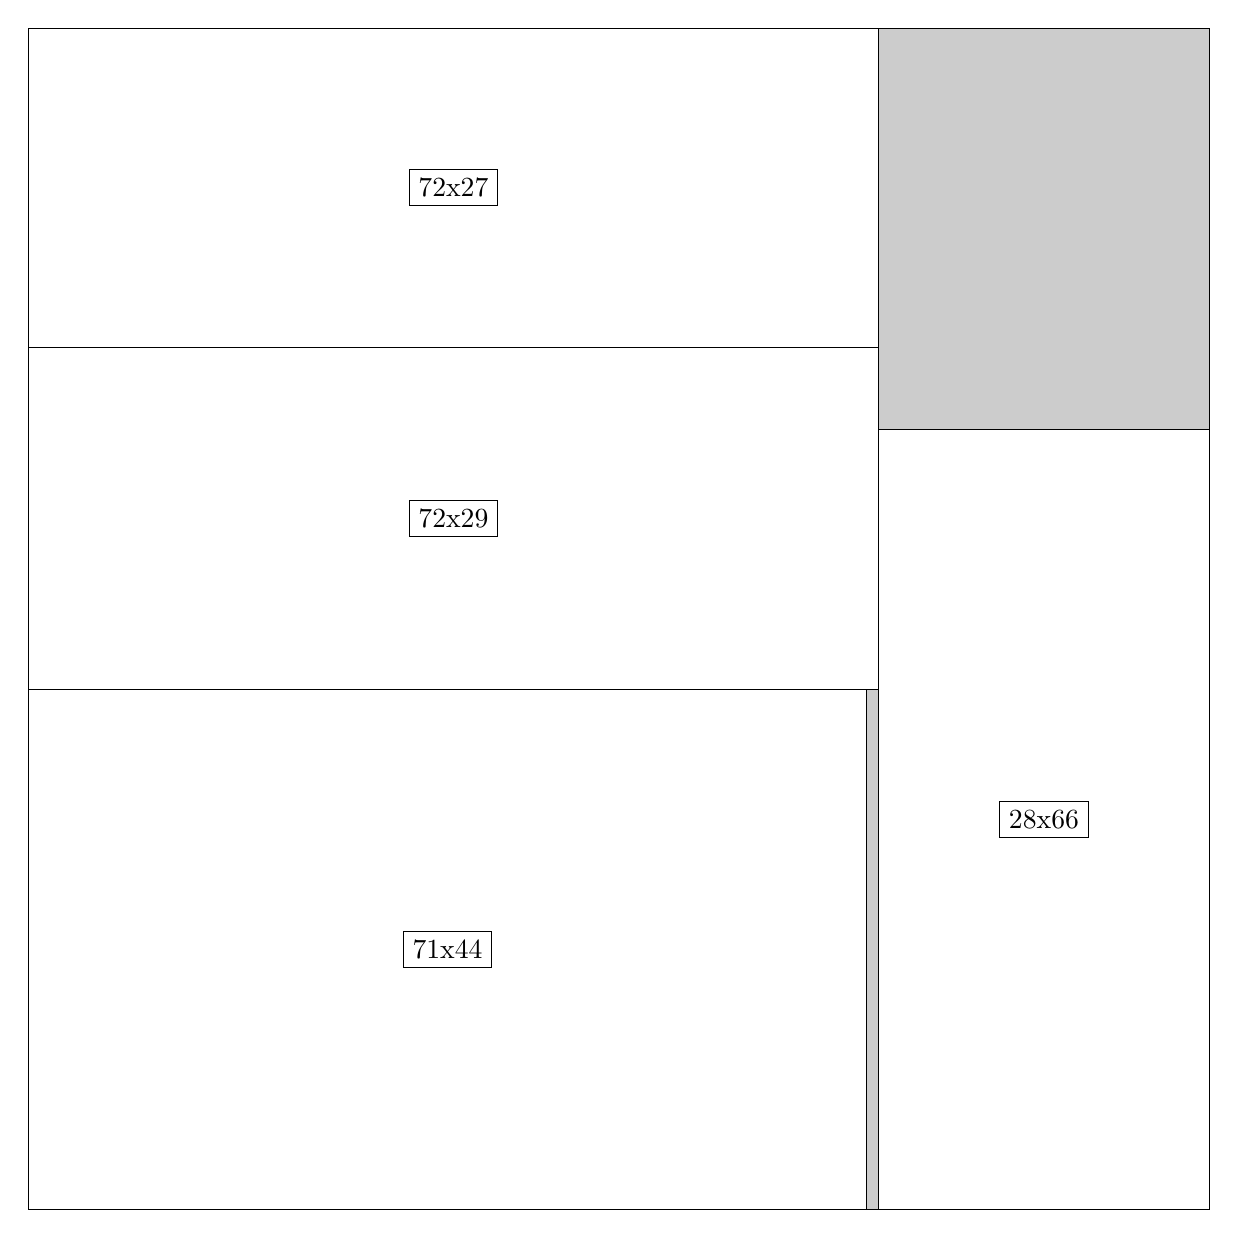
\begin{tikzpicture}[shorten >=1pt,scale=1.0,every node/.style={scale=1.0},->]
\tikzstyle{vertex}=[circle,fill=black!25,minimum size=14pt,inner sep=0pt]
\filldraw[fill=gray!40!white, draw=black] (0,0) rectangle (15.0,15.0);
\foreach \name/\x/\y/\w/\h in {71x44/0.0/0.0/10.65/6.6,72x29/0.0/6.6/10.799999999999999/4.35,72x27/0.0/10.95/10.799999999999999/4.05,28x66/10.799999999999999/0.0/4.2/9.9}
\filldraw[fill=white!40!white, draw=black] (\x,\y) rectangle node[draw] (\name) {\name} ++(\w,\h);
\end{tikzpicture}


w =71 , h =44 , x =0 , y =0 , v =3124
\par
w =72 , h =29 , x =0 , y =44 , v =2088
\par
w =72 , h =27 , x =0 , y =73 , v =1944
\par
w =28 , h =66 , x =72 , y =0 , v =1848
\par
\newpage


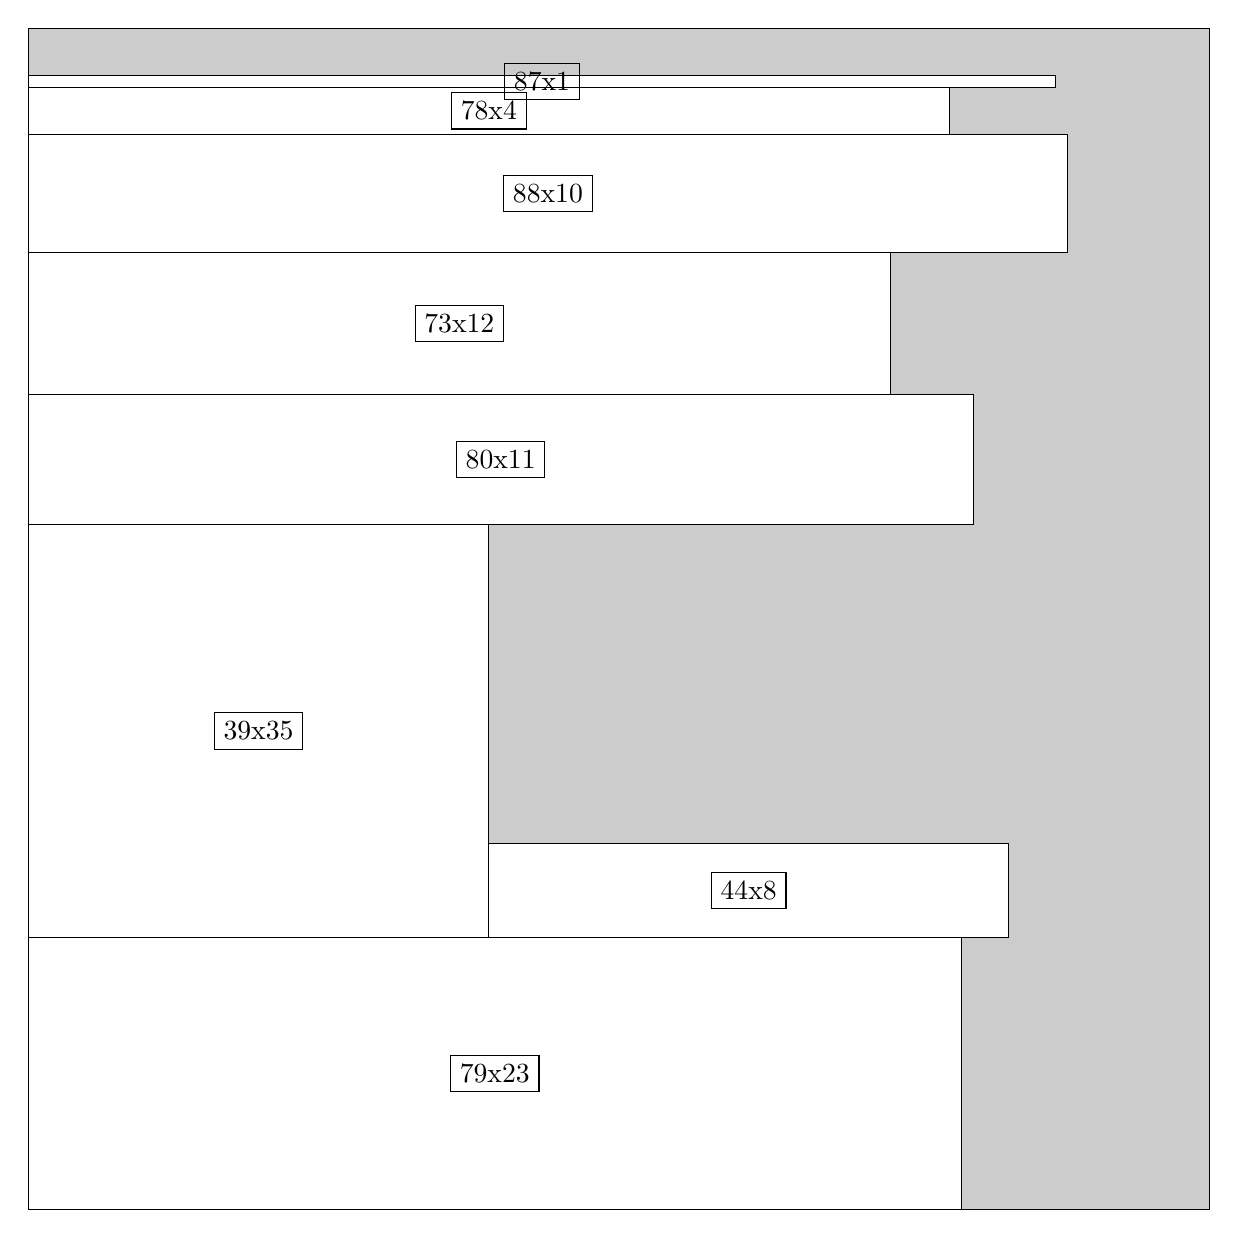
\begin{tikzpicture}[shorten >=1pt,scale=1.0,every node/.style={scale=1.0},->]
\tikzstyle{vertex}=[circle,fill=black!25,minimum size=14pt,inner sep=0pt]
\filldraw[fill=gray!40!white, draw=black] (0,0) rectangle (15.0,15.0);
\foreach \name/\x/\y/\w/\h in {79x23/0.0/0.0/11.85/3.4499999999999997,39x35/0.0/3.4499999999999997/5.85/5.25,44x8/5.85/3.4499999999999997/6.6/1.2,80x11/0.0/8.7/12.0/1.65,73x12/0.0/10.35/10.95/1.7999999999999998,88x10/0.0/12.15/13.2/1.5,78x4/0.0/13.65/11.7/0.6,87x1/0.0/14.25/13.049999999999999/0.15}
\filldraw[fill=white!40!white, draw=black] (\x,\y) rectangle node[draw] (\name) {\name} ++(\w,\h);
\end{tikzpicture}


w =79 , h =23 , x =0 , y =0 , v =1817
\par
w =39 , h =35 , x =0 , y =23 , v =1365
\par
w =44 , h =8 , x =39 , y =23 , v =352
\par
w =80 , h =11 , x =0 , y =58 , v =880
\par
w =73 , h =12 , x =0 , y =69 , v =876
\par
w =88 , h =10 , x =0 , y =81 , v =880
\par
w =78 , h =4 , x =0 , y =91 , v =312
\par
w =87 , h =1 , x =0 , y =95 , v =87
\par
\newpage


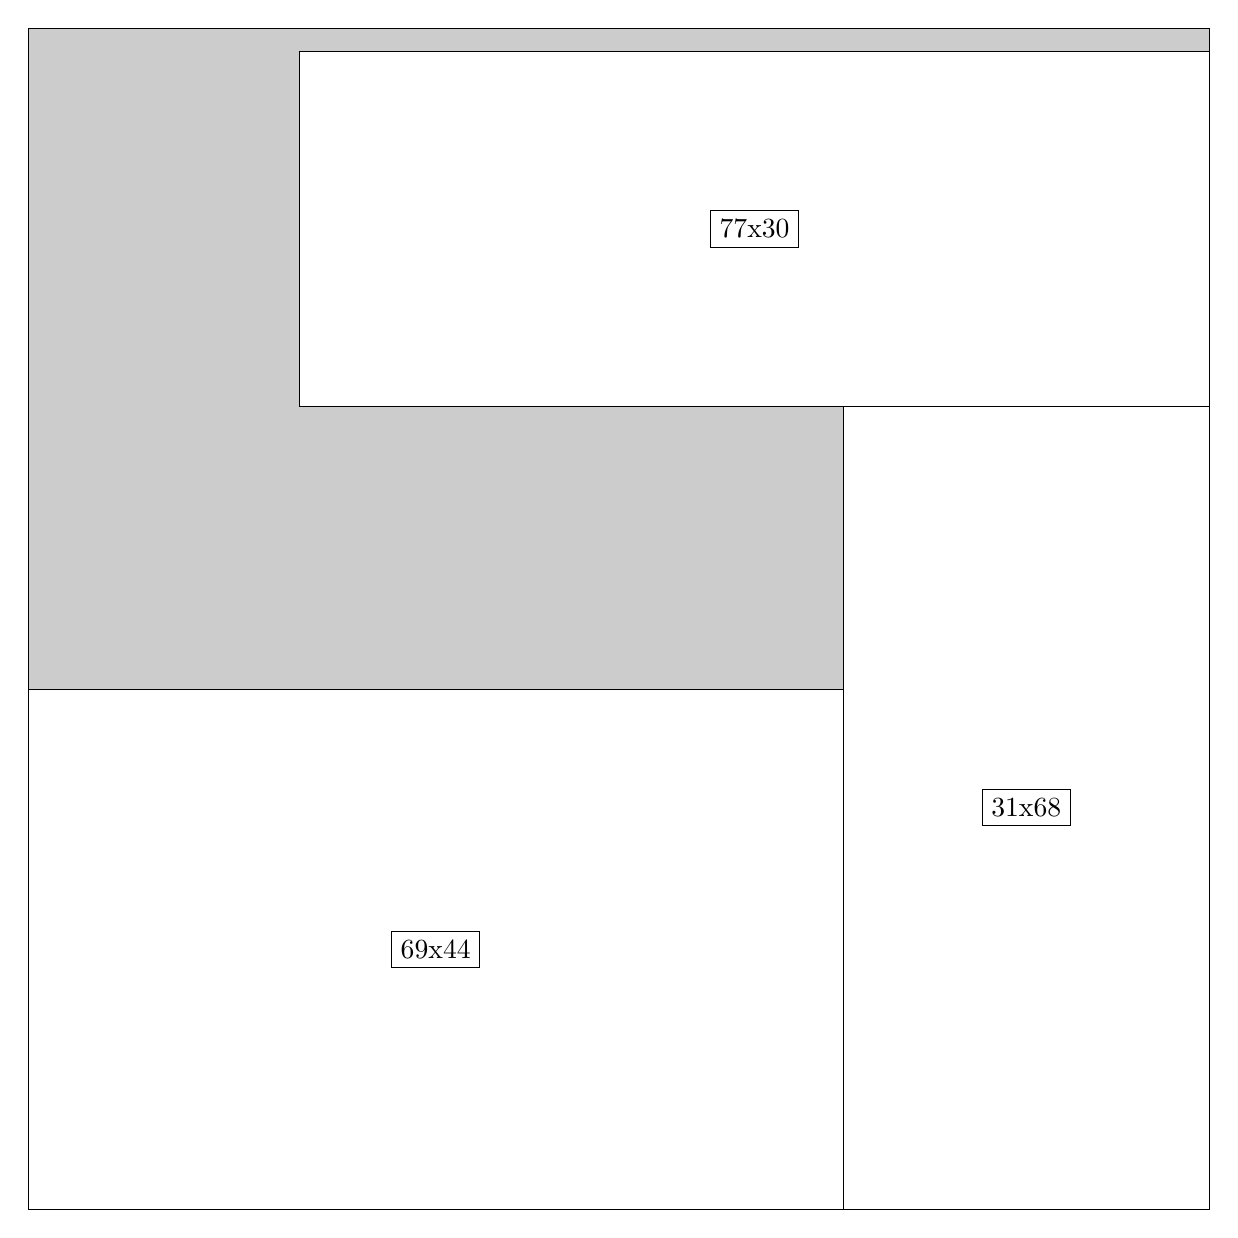
\begin{tikzpicture}[shorten >=1pt,scale=1.0,every node/.style={scale=1.0},->]
\tikzstyle{vertex}=[circle,fill=black!25,minimum size=14pt,inner sep=0pt]
\filldraw[fill=gray!40!white, draw=black] (0,0) rectangle (15.0,15.0);
\foreach \name/\x/\y/\w/\h in {69x44/0.0/0.0/10.35/6.6,77x30/3.4499999999999997/10.2/11.549999999999999/4.5,31x68/10.35/0.0/4.6499999999999995/10.2}
\filldraw[fill=white!40!white, draw=black] (\x,\y) rectangle node[draw] (\name) {\name} ++(\w,\h);
\end{tikzpicture}


w =69 , h =44 , x =0 , y =0 , v =3036
\par
w =77 , h =30 , x =23 , y =68 , v =2310
\par
w =31 , h =68 , x =69 , y =0 , v =2108
\par
\newpage


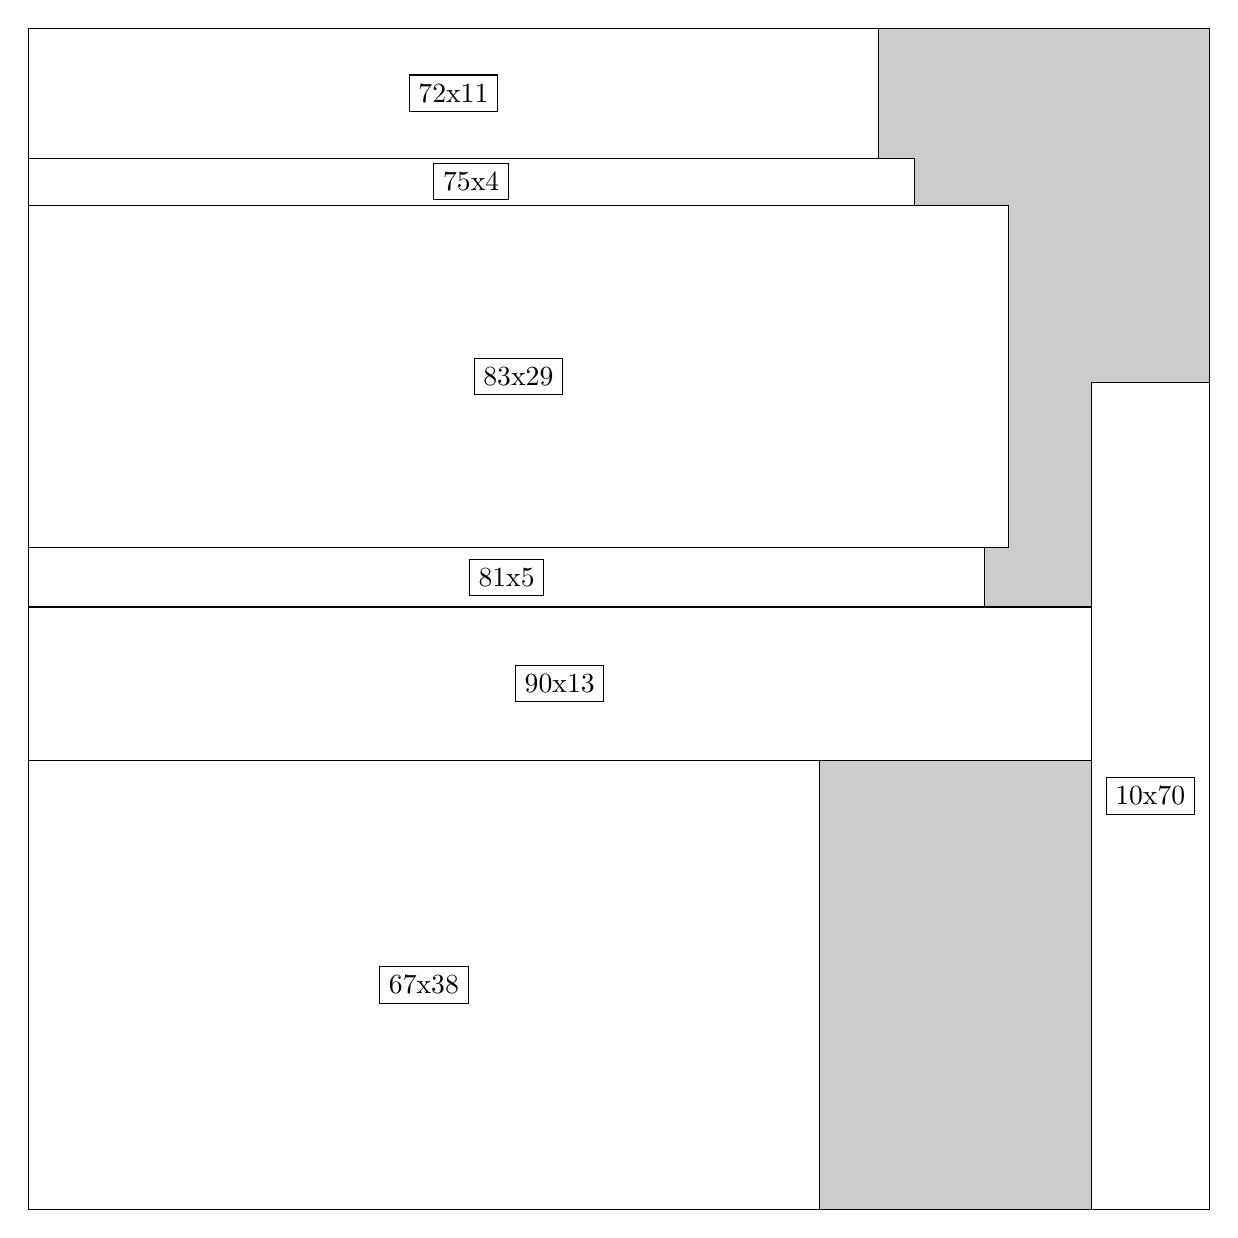
\begin{tikzpicture}[shorten >=1pt,scale=1.0,every node/.style={scale=1.0},->]
\tikzstyle{vertex}=[circle,fill=black!25,minimum size=14pt,inner sep=0pt]
\filldraw[fill=gray!40!white, draw=black] (0,0) rectangle (15.0,15.0);
\foreach \name/\x/\y/\w/\h in {67x38/0.0/0.0/10.049999999999999/5.7,83x29/0.0/8.4/12.45/4.35,90x13/0.0/5.7/13.5/1.95,72x11/0.0/13.35/10.799999999999999/1.65,10x70/13.5/0.0/1.5/10.5,81x5/0.0/7.6499999999999995/12.15/0.75,75x4/0.0/12.75/11.25/0.6}
\filldraw[fill=white!40!white, draw=black] (\x,\y) rectangle node[draw] (\name) {\name} ++(\w,\h);
\end{tikzpicture}


w =67 , h =38 , x =0 , y =0 , v =2546
\par
w =83 , h =29 , x =0 , y =56 , v =2407
\par
w =90 , h =13 , x =0 , y =38 , v =1170
\par
w =72 , h =11 , x =0 , y =89 , v =792
\par
w =10 , h =70 , x =90 , y =0 , v =700
\par
w =81 , h =5 , x =0 , y =51 , v =405
\par
w =75 , h =4 , x =0 , y =85 , v =300
\par
\newpage


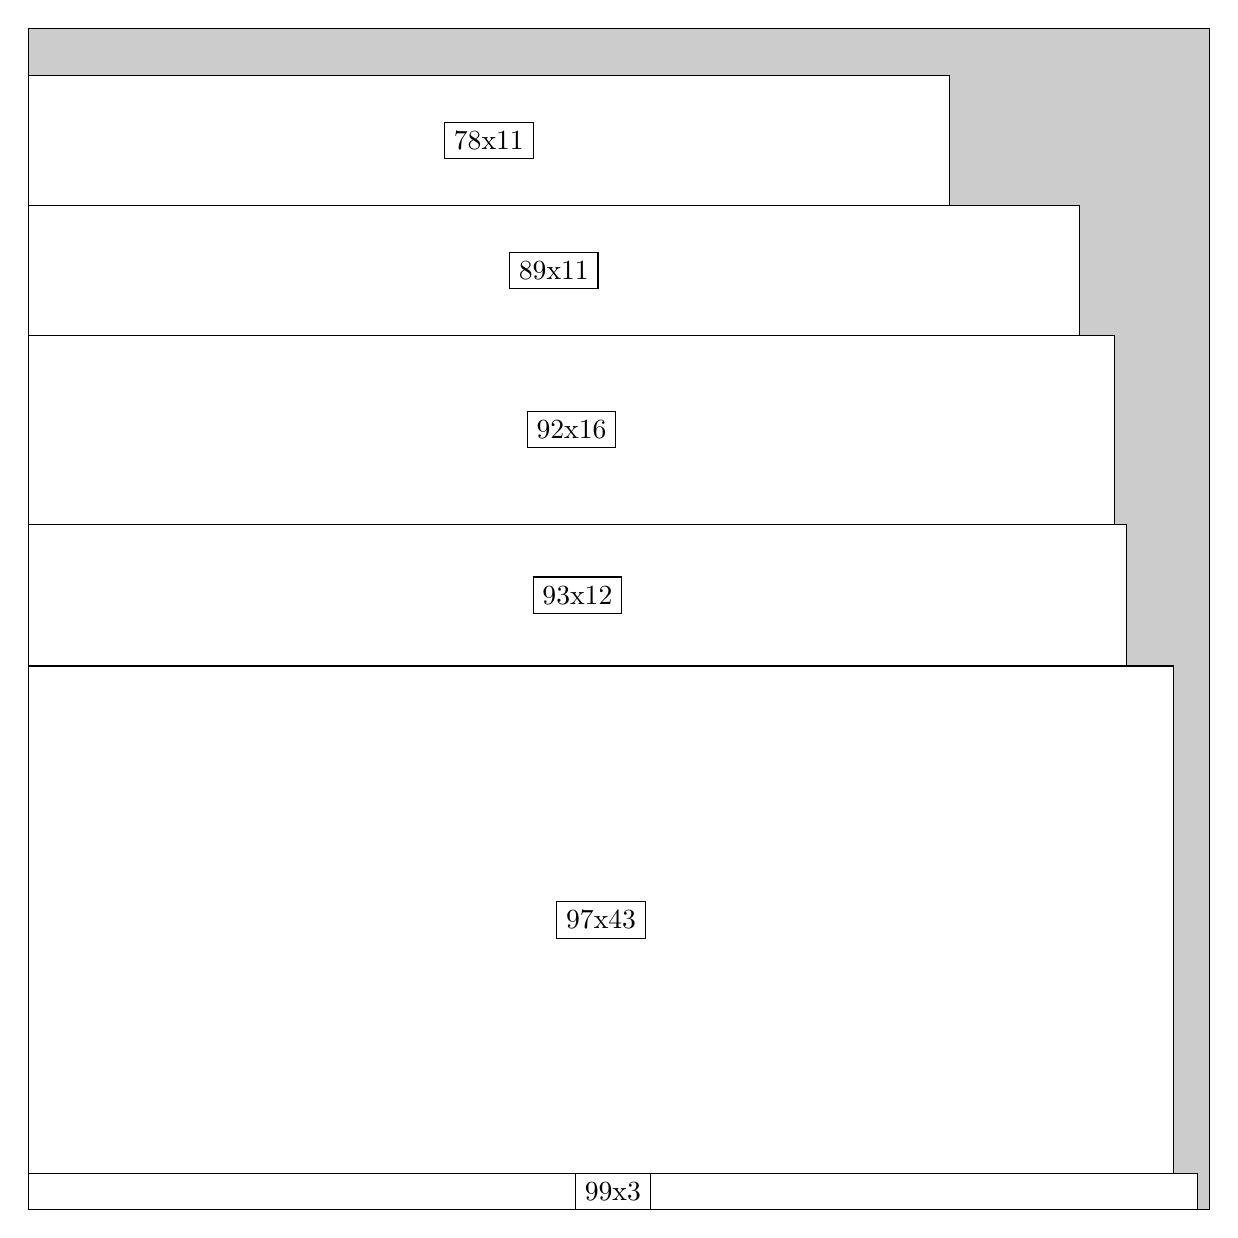
\begin{tikzpicture}[shorten >=1pt,scale=1.0,every node/.style={scale=1.0},->]
\tikzstyle{vertex}=[circle,fill=black!25,minimum size=14pt,inner sep=0pt]
\filldraw[fill=gray!40!white, draw=black] (0,0) rectangle (15.0,15.0);
\foreach \name/\x/\y/\w/\h in {97x43/0.0/0.44999999999999996/14.549999999999999/6.45,89x11/0.0/11.1/13.35/1.65,92x16/0.0/8.7/13.799999999999999/2.4,93x12/0.0/6.8999999999999995/13.95/1.7999999999999998,78x11/0.0/12.75/11.7/1.65,99x3/0.0/0.0/14.85/0.44999999999999996}
\filldraw[fill=white!40!white, draw=black] (\x,\y) rectangle node[draw] (\name) {\name} ++(\w,\h);
\end{tikzpicture}


w =97 , h =43 , x =0 , y =3 , v =4171
\par
w =89 , h =11 , x =0 , y =74 , v =979
\par
w =92 , h =16 , x =0 , y =58 , v =1472
\par
w =93 , h =12 , x =0 , y =46 , v =1116
\par
w =78 , h =11 , x =0 , y =85 , v =858
\par
w =99 , h =3 , x =0 , y =0 , v =297
\par
\newpage


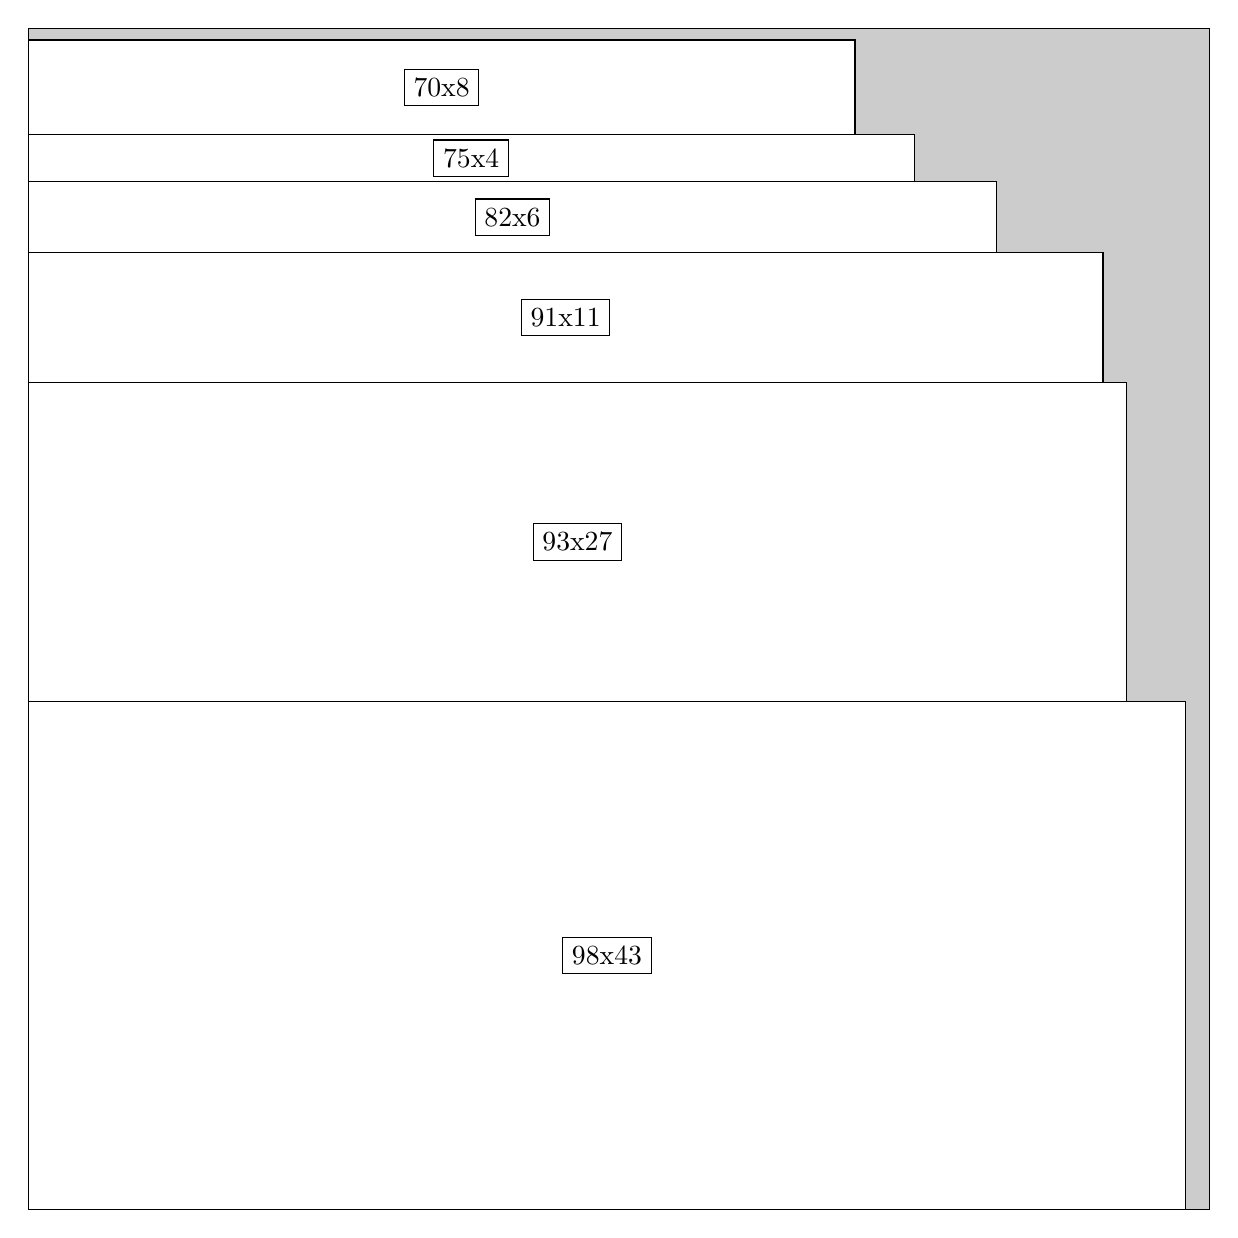
\begin{tikzpicture}[shorten >=1pt,scale=1.0,every node/.style={scale=1.0},->]
\tikzstyle{vertex}=[circle,fill=black!25,minimum size=14pt,inner sep=0pt]
\filldraw[fill=gray!40!white, draw=black] (0,0) rectangle (15.0,15.0);
\foreach \name/\x/\y/\w/\h in {98x43/0.0/0.0/14.7/6.45,93x27/0.0/6.45/13.95/4.05,91x11/0.0/10.5/13.65/1.65,70x8/0.0/13.65/10.5/1.2,82x6/0.0/12.15/12.299999999999999/0.8999999999999999,75x4/0.0/13.049999999999999/11.25/0.6}
\filldraw[fill=white!40!white, draw=black] (\x,\y) rectangle node[draw] (\name) {\name} ++(\w,\h);
\end{tikzpicture}


w =98 , h =43 , x =0 , y =0 , v =4214
\par
w =93 , h =27 , x =0 , y =43 , v =2511
\par
w =91 , h =11 , x =0 , y =70 , v =1001
\par
w =70 , h =8 , x =0 , y =91 , v =560
\par
w =82 , h =6 , x =0 , y =81 , v =492
\par
w =75 , h =4 , x =0 , y =87 , v =300
\par
\newpage


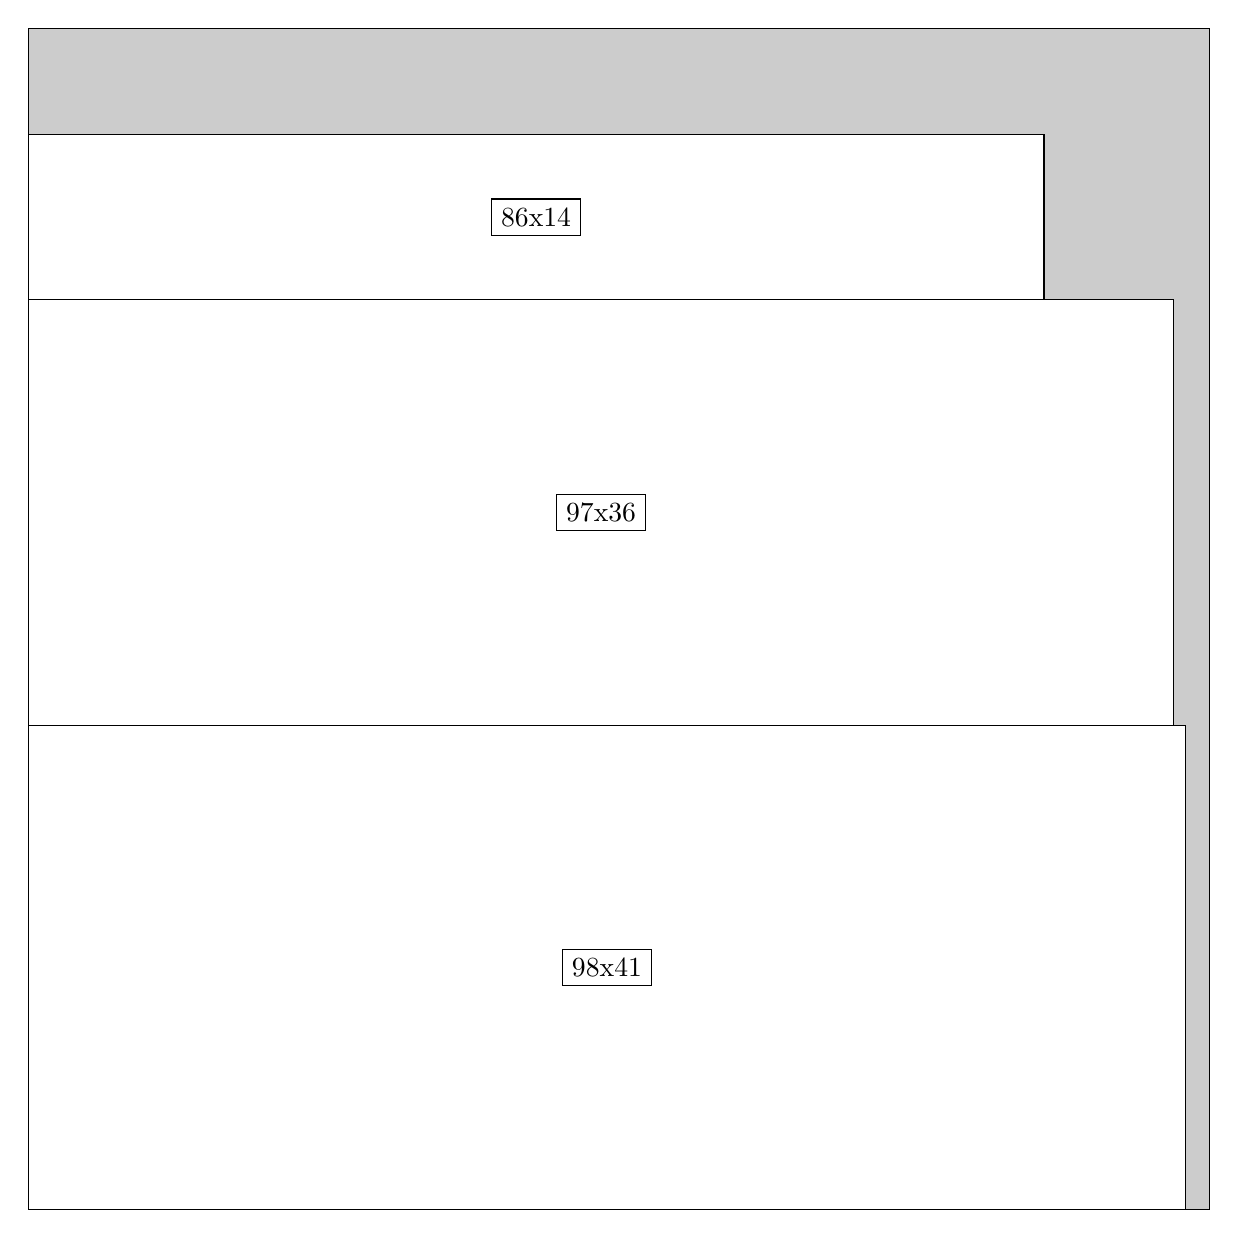
\begin{tikzpicture}[shorten >=1pt,scale=1.0,every node/.style={scale=1.0},->]
\tikzstyle{vertex}=[circle,fill=black!25,minimum size=14pt,inner sep=0pt]
\filldraw[fill=gray!40!white, draw=black] (0,0) rectangle (15.0,15.0);
\foreach \name/\x/\y/\w/\h in {98x41/0.0/0.0/14.7/6.1499999999999995,97x36/0.0/6.1499999999999995/14.549999999999999/5.3999999999999995,86x14/0.0/11.549999999999999/12.9/2.1}
\filldraw[fill=white!40!white, draw=black] (\x,\y) rectangle node[draw] (\name) {\name} ++(\w,\h);
\end{tikzpicture}


w =98 , h =41 , x =0 , y =0 , v =4018
\par
w =97 , h =36 , x =0 , y =41 , v =3492
\par
w =86 , h =14 , x =0 , y =77 , v =1204
\par
\newpage


\end{document}